\subsection{Coverage and resilience of routing}
\todo[inline]{PROBLEM - COVERAGE}
\subsubsection{Coverage}

\begin{definition}[Composite task coverage]
	\todo[inline]{DO we need this? This is covered by having the atomic task quality in composite task quality}
	Given a composite task $\varCompositeTask{}{}$, and completes or partially completes this task $\varCompositeTask{}{*} \subseteq \varCompositeTask{}{}$ then the \textit{composite task coverage} of $\varCompositeTask{}{}$ is the fraction of successfully completed atomic tasks of the composite task.
	\begin{equation}
		\functionCompositeTaskCoverage{}{} = \frac{
			\funcSize{\varCompositeTask{}{*}
			}
		}{
			\funcSize{\varCompositeTask{}{}
			}
		}
	\end{equation}
\end{definition}


\subsubsection{Route adaptation}
Figure \ref{fig:wsnhierarchicalresolution} shows one of the possible modes of hierarchical networking that can be formed by the agent system through per-agent local neighbourhood learning. The initial agent passes requests through smaller and smaller neighbourhoods until the granulaity of the data meets that of the request

\begin{figure}[]
	\centering
	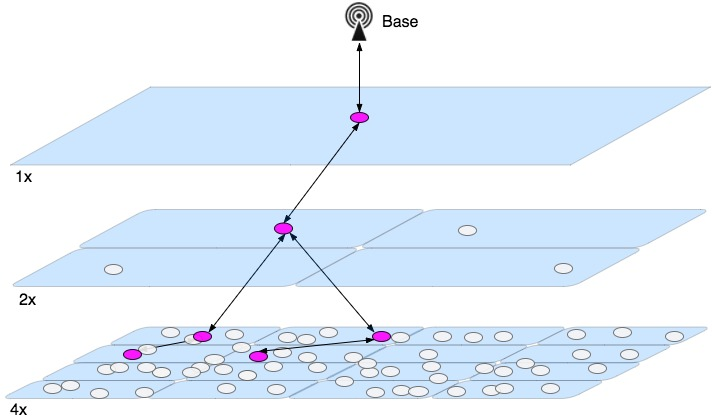
\includegraphics[width=0.5\linewidth]{WSN_hierarchical_resolution}
	\caption{Agent system hierarchical neighbourhood resolution}
	\label{fig:wsnhierarchicalresolution}
\end{figure}
In Figure \ref{fig:wsnsimulationmapfailureadaptation}, the first figure shows a set of agents aggregating data across a defined granularity geographical area using their learned neighbourhoods. In the second we see the adaptation of each agents local neighbourhood as they individually react to device failures
\begin{figure}[]
	\centering
	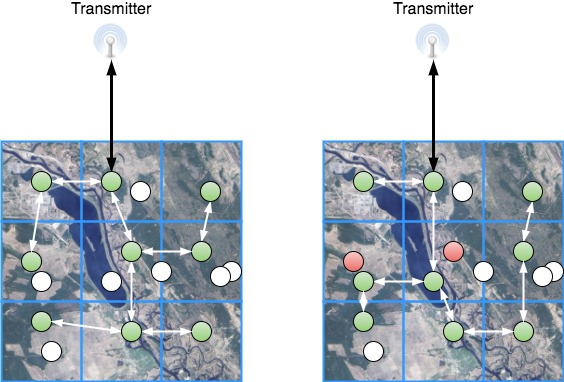
\includegraphics[width=0.5\linewidth]{WSN_simulation_map_failure_adaptation}
	\caption{WSN simulation failure adaptation}
	\label{fig:wsnsimulationmapfailureadaptation}
\end{figure}

